\documentclass[conference]{IEEEtran}
%\IEEEoverridecommandlockouts
% The preceding line is only needed to identify funding in the first footnote. If that is unneeded, please comment it out.
\usepackage{amsmath,amssymb,amsfonts}
%\usepackage{algorithmic}
\usepackage{graphicx}
\usepackage{textcomp}
\usepackage{xcolor}
\usepackage{float}
\usepackage{url}
\usepackage{multirow}
\usepackage{biblatex}
\def\BibTeX{{\rm B\kern-.05em{\sc i\kern-.025em b}\kern-.08em
    T\kern-.1667em\lower.7ex\hbox{E}\kern-.125emX}}

\newcommand{\figref}[1]{Figure~\ref{#1}} 
\newcommand{\secref}[1]{Section~\ref{#1}}
\newcommand{\tabref}[1]{Table~\ref{#1}}

% Fix some overfull hboxes
\setlength{\tabcolsep}{4pt}

% Allow linebreaks at underscores
\renewcommand\_{\textunderscore\allowbreak}
    
\bibliography{Paper}
\begin{document}

\title{TSCH: A look at reliability and energy requirements}

\author{\IEEEauthorblockN{Gabriele Paris}
\IEEEauthorblockA{\textit{Dept physic} \\
\textit{University of Antwerp}\\
Antwerp, Belgium \\
gabriele.paris@student.uantwerpen.be}
\and
\IEEEauthorblockN{Pieter Hendriks}
\IEEEauthorblockA{\textit{Dept computer science} \\
\textit{University of Antwerp}\\
Antwerp, Belgium \\
pieter.hendriks@student.uantwerpen.be}
}

\maketitle

\begin{abstract}
In this paper, we assess the energy performance of TSCH and 6TiSCH using the Contiki-NG operating system on Zolertia RE-mote (Rev. B) nodes.\\
These boards are part of the IoT hardware family, and they allow for the creation of a network minimizing energy consumption.\\
We perform different experiments aiming to evaluate various parameters such as energy consumption or latency between the boards in a two node network.\\
We consider three different analyses in this paper. First, we compare the energy use when using a full network stack to the energy use when only having the TSCH MAC layer enabled. Second, we look at the TSCH association process and analyze the time and energy required for each node. Finally, we consider the impact distancing the nodes from each other has on network reliability and energy consumption. 
Comparing the energy usage we found that in a MAC only configuration the leaf and root node have the same energy consumption, such value diminishes for both of them if the full stack is enabled. 
The join process is mostly impacted by the length of the hopping sequence, though the EB period also has significant impact. Distance between the nodes starts impacting performance noticeably (from our tested distances) at 50m, leading to completely unacceptable performance at low TX powers when reaching 100m.
\end{abstract}

\begin{IEEEkeywords}
6TiSCH, Contiki-NG, Energest, IEEE 802.15.4, Power Consumption, Range, Time Slotted Channel Hopping, 6TiSCH, TSCH, Zolertia
\end{IEEEkeywords}

\section{Introduction}
The IETF IPv6 over the TSCH mode of IEEE802.15.4e (6TiSCH) working group has standardized a set of protocols to enable low power industrial-grade IPv6 networks. 6TiSCH proposes a protocol stack rooted in the Time Slotted Channel Hopping (TSCH) mode of the IEEE802.15.4-2015 standard, a scheme aiming to guarantee network reliability by keeping nodes time-synchronised at the MAC layer. The latter is accomplished by scheduling, therefore nodes must remain time synchronised throughout the network deployment’s life-time. To this end, nodes periodically exchange Enhanced Beacon (EB) packets\cite{6tischDef}. It supports multi-hop topologies with the IPv6 Routing Protocol for Low-Power and Lossy Networks (RPL) routing protocol, and is IPv6-ready through 6LoWPAN\cite{6tischDef}.

Contiki-NG is an operating system for resource-constrained devices in the Internet of Things. Contiki-NG contains an RFC-compliant, low-power IPv6 communication stack, enabling Internet connectivity. The system runs on a variety of platforms based on energy-efficient architectures such as the ARM Cortex-M3/M4 and the Texas Instruments MSP430. The code footprint is on the order of a 100 kB, and the memory usage can be configured to be as low as 10 kB. 

This paper serves as an initial look at the performance of TSCH on the Contiki-NG operating system. We study the following cases:
\begin{itemize}
\item Energy consumption of TSCH network stack vs 6TiSCH network stack
\item Time taken for and energy used during node association with an established TSCH network
\item Measure the impact of distance between nodes on energy use and network reliability
\end{itemize}

The hardware in use are Zolertia RE-Mote boards, designed jointly with universities and industry partners in RERUM European project, to ease the development of private and secure applications for IoT and Smart City applications.\\
The RE-Mote packs several onboard resources, like an accurate time keeper real time clock (RTC), external watchdog timer (WDT) to force an embedded microprocessor or microcontroller to reset in case of loop, Micro-SD, RF switch, and a Shutdown mode to reduce its power consumption down to 150nA\cite{contiki-NGWiki}.

The paper is subdivided into three main sections: in the first one, we will compare the energy consumption of the leaf and root node (LLC) at first using up to the MAC TSCH layer, and then using the full stack.\\
In the second section, we will analyze the TSCH joining process and relative energy consumption. Further, in the final section, we will assess the performance of the TSCH mode over various distances.



\section{Related Work}
\subsection{Accurate energy consumption using Energest}
In \secref{section:task1} of this paper, we focus on the analysis of the energy consumption between leaf and root node. This analysis can be done by knowing different parameters like current, voltage, and time. Voltage is always fixed at $3.3V$ due to the power supply and voltage regulator on the board, current should instead be correctly provided in the board datasheet, previous works have shown that real current consumption values are different from the datasheet provided ones\cite{EnergyConsumption}. In this paper, we are going to use such current measurements to determine the energy consumption.
\subsection{Throughput Analysis} S. Lee et al present an analysis of the throughput performance of TSCH networks. They show which parameters of the TSCH networks (node count, hop count) influence the throughput metric in what way. They concluded that throughput capability of the network increases as the node count increases. The throughput capability drops when the hop count increases. Our research focuses on different performance characteristics of the TSCH implementation (energy efficiency rather than throughput), while varying different variables and can be useful alongside these results\cite{ThroughputEvaluation}. 
\subsection{Join Process Performance} D. De Guglielmo et al analyse the time it takes for nodes to associate with an existing TSCH network. Their work focuses on the time taken for nodes to associate to the network and finds that the amount of channels in the hopping sequence is the most important factor\cite{JoinProcess}. Our research additionally considers the energy states nodes are in during the join process. 

\section{Analysing the 6TiSCH energy consumption}
\label{section:task1}

\subsection{Introduction} 
\label{section:t1_intro}
In the first analysis, we compared the energy consumption during a certain time period of the entire 6TiSCH stack to when only enabling the TSCH MAC layer (without link-layer security) after network convergence.
The full stack can be seen as in \figref{fig:6tischStack}.


For both analyses, we report on the consumption of the root and the leaf node separately.
Following we remark differences in energy consumption between the root and the leaf node in the two different scenarios.
The TSCH mode for medium access control (MAC) included in the standard IEEE 802.15.4 has been designed as the multichannel MAC protocol for Low-power and lossy networks (LLNs), a key component of the IoT. Its flexibility makes the TSCH mode a very promising candidate for the future of the MAC layer in LLNs. As such, its performance under different conditions must be assessed, so that accurate guidelines for its application can be drawn\cite{TSCHExperimentEval}.
\begin{figure}[htbp]
	\centering
	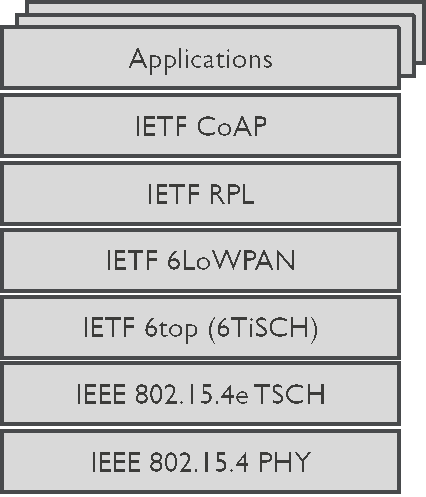
\includegraphics[width=.25\textwidth,keepaspectratio]{figures/6TiSCH-Protocol-Stack.png}
	\caption{6TiSCH Protocol Stack\cite{TimeCritical6tisch}.}
	\label{fig:6tischStack}
\end{figure}


the physical setup of the experiment consists of two Zolertia  Remote RevB boards placed at a fixed distance of approximately 20 cm as shown in \figref{fig:exp1Topology}. There is nothing between the boards hindering communication.

\begin{figure}[htbp]
	\centering
	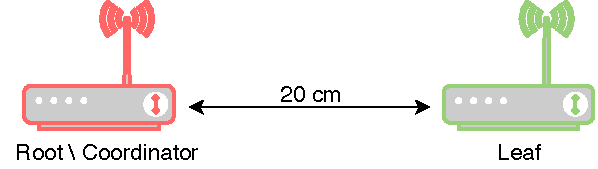
\includegraphics[width=.35\textwidth,keepaspectratio]{figures/exp1Topology.pdf}
	\caption{Network topology for 6TiSCH energy consumption analysis.}
	\label{fig:exp1Topology}
\end{figure}
The basic setup for the following analysis is a root (coordinator) node and a leaf node that exchange the same amount of data packets.
Both nodes are configured to measure the energy consumption by the Energest\footnote{https://github.com/contiki-ng/contiki-ng/wiki/Documentation:-Energest} module available in Contiki-ng\footnote{https://github.com/contiki-ng}.
The Energest module can be used to implement lightweight, software-based energy estimation approach for resource-constrained IoT devices. By tracking the time various hardware states such as the radio is turned on, and by knowing the power consumption of the state, it is possible to estimate the energy consumption\cite{contiki-NGWiki}.
The energy consumption is measured referring to the following formula:
\begin{equation}
	E_{tot}=\sum_{s \in state}^{N_{s}}E_{s}=\sum_{s \in state}^{N_{s}}I_s  \cdot V_{cc} \cdot t
\end{equation}

Where $V_{cc}$ is the supply voltage, fixed as a constant at the value $3.3V$, $I_s$ is provided by the Table \tabref{tab:CurrentConsumption} column \textit{Device profiling}\cite{EnergyConsumption} chosen because more accurate than the one provided by the CC2538 datasheet, and $t$ is measured using Energest.

All measurements are performed in a span of 15 minutes each.
\begin{table}[htbp]
	\begin{center}
		\begin{tabular}{ccc}
			\hline
			\textbf{State}    & \textbf{\begin{tabular}[c]{@{}c@{}}CC2538\\ datasheet\end{tabular}} & \textbf{\begin{tabular}[c]{@{}c@{}}Device\\ profiling\end{tabular}} \\ \hline
			\textbf{CPU}      & 20 mA                                                               & 15.35mA                                                             \\
			\textbf{LPM}      & 0.6 mA                                                              & 9.59 mA                                                             \\
			\textbf{Deep LPM} & 0.0013 mA                                                           & 2.58 mA                                                             \\
			\textbf{LISTEN}   & 24 mA                                                               & 28.32 mA                                                            \\
			\textbf{Rx}       & 27 mA                                                               & 30.14 mA                                                            \\
			\textbf{Tx}       & 34 mA                                                               & 31.12 mA                                                            \\ \hline
		\end{tabular}
	\end{center}
	\caption{Comparison between values from the datasheet and N6705B DC Power Analyzer radio.\cite{EnergyConsumption}}
	\label{tab:CurrentConsumption}
\end{table}
\subsection{Only TSCH MAC layer}
In the first part of the experiment, we used only the stack till the MAC layer (TSCH) as shown in \figref{fig:6tischStack}.
In TSCH networks, every node follows a time-synchronized schedule. This schedule instructs every node about exactly what to do and avoids wasting valuable energy. The TSCH schedule is divided into time slots. The duration of a time slot is typically 10 ms or 15 ms and sufficient to transmit a packet of the maximum size of 127 bytes, immediately followed by an optional acknowledgment frame indicating that the packet was successfully received. Multiple time slots are grouped into a slot frame, and the size of a slot frame defines the width of the schedule. These slot frames repeat continuously over time. TSCH also allows one to use multiple frequencies, leading to a two-dimensional matrix of cells. The number of available frequencies actually determines the height of the schedule\cite{AccurateEnergyTSCH}.

We proceeded as explained in the setup to measure the energy consumption between leaf and root node.\\
Results, measured after network convergence, are reported in \tabref{tab:MACOnly}.

\begin{table}[htbp]
	\centering
	\begin{tabular}{llllll}
		\hline
		\textbf{Node} & \multicolumn{1}{c}{\textbf{CPU}} & \multicolumn{1}{c}{\textbf{LPM}} & \multicolumn{1}{c}{\textbf{Deep}} & \multicolumn{1}{c}{\textbf{Tx}} & \multicolumn{1}{c}{\textbf{Rx}} \\ \hline
		\textbf{Leaf} & 3.330 mJ                         & 314.385 mJ                       & 85.143 mJ                         & 1.132 mJ                        & 993.527 mJ                      \\
		\textbf{Root} & 3.330 mJ                         & 314.385 mJ                       & 85.143 mJ                         & 1.132 mJ                        & 993.527 mJ                      \\ \hline
	\end{tabular}
	\caption{Average power consumption comparison between root and leaf node per state, TSCH MAC only.}
	\label{tab:MACOnly}
\end{table}
What we can see is that data from root and leaf nodes show no variation, and the energy consumed from both of them is the same.\\
In a TSCH network The root needs to control the way the network is formed, including how new nodes join and how already joined nodes advertise the presence of the network, this is all encoded in the TSCH RFC\footnote{https://tools.ietf.org/html/rfc7554}.\\
The root node during network convergence needs to:
\begin{itemize}
	\item Define the Information Elements included in the Enhanced Beacons, advertising the presence of the network;
	\item for a new node define rules to process and filter received EBs;
	\item Define the joining procedure.  This might include a mechanism to assign a unique 16-bit address to a node and the management of initial keying material;
	\item Define a mechanism to secure the joining process and the subsequent optional process of scheduling more communication cells.
\end{itemize}
After the network has been formed it must be mantained, this implies that the root node must:
\begin{itemize}
	\item Manage each node's time source neighbor;
	\item Define a mechanism for a node to update the join priority it announces in its EB;
	\item Schedule transmissions of EBs to advertise the presence of the network.
\end{itemize}
We can therefore say that, atleast for two node comunicating for such time, after network convergence, the workload on the root is not enought to show a difference in energy consumption during the stated time spam.
\subsection{Full stack}
The next experiment is as cited in \secref{section:t1_intro} related to the energy consumption once the full 6TiSCH stack has been enabled (except for the security layer).\\
The setup of this experiment is the same to the previous one.
Two boards 20cm apart from each other (\ref{fig:exp1Topology}) are running the same source code.

In this scenario, we have a coordinator node and a leaf node.\\
No messages are exchanged between the two if not for standard 6TiSCH service messages.\\
We proceeded as explained in the setup to measure the energy consumption between leaf and root node.\\
Results are reported in \tabref{tab:FullStack}.
\begin{table}[htbp]
	\centering
	\begin{tabular}{llllll}
		\hline
		\textbf{Node} &
		\multicolumn{1}{c}{\textbf{CPU}} &
		\multicolumn{1}{c}{\textbf{LPM}} &
		\multicolumn{1}{c}{\textbf{Deep}} &
		\multicolumn{1}{c}{\textbf{Tx}} &
		\multicolumn{1}{c}{\textbf{Rx}} \\ \hline
		\textbf{Leaf} &
		5.00 mJ &
		313.341 mJ &
		85.143 mJ &
		80.121 mJ &
		98.362 mJ \\
		\textbf{Root} &
		3.890 mJ &
		310.560 mJ &
		84.209 mJ &
		0 mJ &
		33.879 mJ \\ \hline
	\end{tabular}
	\caption{Average power consumption per state between root and leaf node, full 6TiSCH  stack.}
	\label{tab:FullStack}
\end{table}
\subsection{Final comparison}
As a final comparison, we compared the total energy usage between root and leaf nodes in the two configurations.
What we measured has been reported as \tabref{tab:exp1Comparison}.
\begin{table}[htbp]
	\centering
	\begin{tabular}{cll}
		\hline
		\textbf{Node} & \multicolumn{1}{c}{\textbf{MAC only}} & \multicolumn{1}{c}{\textbf{Full stack}} \\ \hline
		\textbf{Leaf} & 1.398 J                                & 0.582 J                                  \\
		\textbf{Root} & 1.398 J                                & 0.433 J                                  \\ \hline
	\end{tabular}
	\caption{Energy comparison between leaf and root node in MAC only and full stack configurations.}
	\label{tab:exp1Comparison}
\end{table}


\section{Energy consumption during the TSCH join process}
\label{section:task2}

\subsection{Introduction} 

A TSCH network advertises through the broadcast of Enhanced Beacons (EB). These are frames that contain the TSCH network properties and reception of such a frame allows a node to attempt to join the TSCH network. In this section, we analyze how long it takes for a node to join an existing TSCH network. We also consider the energy used by the joining node as well as the advertising node.

D. De Guglielmo et al have already done similar work\cite{JoinProcess}. They show that the channel hopping sequence length is the most important factor with regards to the association time. This analysis intends to verify that conclusion (as well as consider the impact of the EB period) and additionally consider the energy used by each node during this association process. 

\subsection{Disclaimer}
\label{sec:t2_discl}
An oversight during the initial experiments for this section caused all the data to be invalid. Since command line defines (set in the Makefile) are used to set the behaviour for the TSCH layer, a recompile of the files setting the configured values is required for them to take effect. Since those files are not changed in between compilations, the Make build system does not automatically re-compile them when the Makefile changes. During our initial experiment set, these were the only changes made in between runs of the software. This was unfortunately uncovered too close to the submission deadline to fully correct.

Initial (incorrect) dataset considered EB periods between 1 and 16 seconds as well as channel hopping sequences between 1 and 16 channels. In order to limit the amount of time needed to perform the experiments, we limit ourselves to EB periods between 1 and 8 seconds and channel hopping sequences between 1 and 4 channels. We further limit the amount of measurements per parameter set to 25 rather than the original 50. 

\subsection{Configuration}

The Contiki-NG operating system offers many options for configuring the TSCH joining process. We briefly discuss the most significant ones below. Any parameters that are changed for our analysis are mentioned in their respective subsections, all others are left as their default value for all performed experiments.

\subsubsection{TSCH\_CONF\_MAX\_JOIN\_PRIORITY}
This parameter sets the maximal allowed depth for a new node attempting to join the network. The TSCH coordinator is at depth 0. For any other node, the depth is defined as 1 + the depth of the node it is trying to connect through (i.e. the advertising node). In our study, we only consider two-node networks, so this parameter is essentially not relevant to our case.

\subsubsection{TSCH\_CONF\_JOIN\_SECURED\_ONLY}
This parameter sets the TSCH layer such that it only allows joining secured TSCH networks. For our experiments, this has been set to disabled. We want to minimize all non-TSCH noise on our measurements. Security layers require additional processing and thus might obscure some of the results we obtain. 

\subsubsection{TSCH\_CONF\_JOIN\_MY\_PANID\_ONLY}
This parameter sets the TSCH layer such that nodes will only join TSCH networks that are advertising the same PAN ID as they were configured with. Any other received EBs (i.e., those with a different PAN ID) are ignored. 

\subsubsection{TSCH\_CONF\_ASSOCIATION\_POLL\_FREQUENCY}
The association poll frequency set by this parameter sets the frequency with which the radio is polled during the association process. This has implications for the energy used by the system, as a higher polling rate would result in higher energy use. However, a higher polling rate might also be able to associate faster. This parameter is left as default in this analysis, but might be interesting to consider in future work.

\subsubsection{TSCH\_CONF\_CHECK\_TIME\_AT\_ASSOCIATION}
Defining this constant enables the functionality that time should be compared to local uptime at association. It will compare the ASN from the EB to the node's own uptime. This can be used to allow nodes to be configured such that they will only connect to networks that were created close to their own boot time. 

\subsubsection{TSCH\_CONF\_INIT\_SCHEDULE\_FROM\_EB} 
\label{t2_initsched}
An EB frame can contain information elements specifying slotframe and link information. This parameter controls whether the node should initialize itself using those information elements.

\subsubsection{TSCH\_CONF\_CHANNEL\_SCAN\_DURATION}

\subsubsection{TSCH\_PACKET\_CONF\_EB\_WITH\_TIMESLOT\_TIMING}
Controls whether the EB frame contains an information element specifying the network's timeslot timings.

\subsubsection{TSCH\_PACKET\_CONF\_EB\_WITH\_HOPPING\_SEQUENCE} 
Controls whether the EB frame contains an information element specifying the network's hopping sequence.

\subsubsection{TSCH\_PACKET\_CONF\_EB\_WITH\_SLOTFRAME\_AND\_LINK}

Controls whether the EB frame contains an information element for the slotframe and link information. This element would be used by the parameter mentioned in \secref{t2_initsched} if that parameter is set.

\subsubsection{TSCH\_CONF\_EB\_PERIOD}
How long the time between EB broadcasts should be. Defaults to 16 seconds. This parameter is varied over our experiments, between 1 and 16 seconds. 

\subsubsection{TSCH\_CONF\_MAX\_EB\_PERIOD} 

The maximal allowed period between EB broadcasts. Defaults to 16 seconds. It imposes an upper limit on the variable mentioned in the previous point.


\subsubsection{TSCH\_CONF\_DEFAULT\_HOPPING\_SEQUENCE}
The default hopping sequence that is configured for the network. This sequence may have duplicate channels and so can have arbitrary length. It is limited by another variable, see \secref{t2_maxlen}.

\subsubsection{TSCH\_CONF\_JOIN\_HOPPING\_SEQUENCE}
This constant determines the hopping sequence a node attempting to join a network will use. By default, this will be the same as the default hopping sequence for the network. It is possible to configure them differently, but our analyses do not use this option.

\subsubsection{TSCH\_CONF\_HOPPING\_SEQUENCE\_MAX\_LEN}
\label{t2_maxlen}
This sets the maximal allowed length for a hopping sequence in the TSCH network. By default it is set to the length of the default hopping sequence. This value is 4 in the standard configuration, but is automatically changed along with the configuration of a different default hopping sequence.

\subsection{Experiment setup}

In this section, we consider two nodes placed 20 cm apart, with nothing between them impeding communication, as in \figref{fig:exp1Topology}. The leaf node will repeatedly associate and disassociate from the TSCH network. The root node will simply wait and output its energy statistics whenever the node associates. The leaf, similarly, will output its time taken and the energy used when association is complete. After the data has been output, the leaf node disassociates from the network and starts over.

We consider the case only where the node disassociates from the network, then immediately reassociates itself. Introducing additional variance by waiting the leaf node for an arbitrary amount of time simply introduces additional noise into the measurements. It is an option that was considered, but discarded. While the effect this has on the measurements simulates a more realistic scenario (node starts listening at a random time), it simply introduces noise into our measurements that were not influenced by the variables we're attempting to isolate. In order to correctly gauge the effect each of the variables we consider has, this additional source of noise was not added.


\subsection{Results}

We see clearly that, regardless of configuration, the leaf node always spends a large amount of time in the RX state. This makes sense as it has to be listening for an EB constantly in order to connect to a network. We also see that, while this happening, it is very rare for the CPU to enter a deep sleep state. Presumably, because of the constant channel switching, the CPU has to perform some computation regularly enough to prevent long deep sleeps. This contrasts heavily with the behaviour observed when the node is connected, where the deep sleep state dominates. This is clear from all data obtained in \secref{section:task3}.



\begin{figure}[htbp]
	\centering
	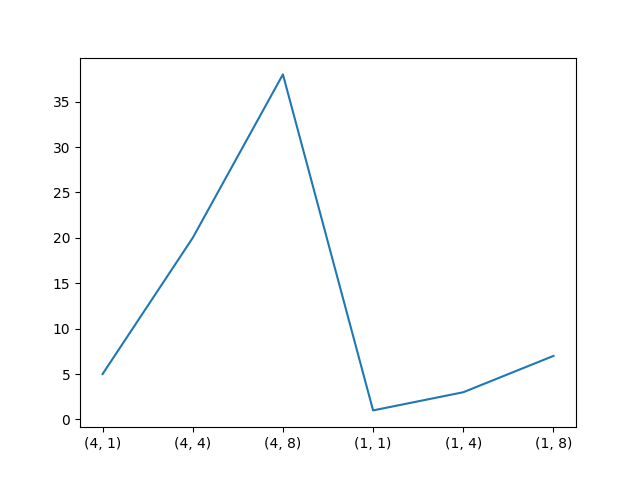
\includegraphics[width=.48\textwidth,keepaspectratio]{figures/times}
	\caption{The average connection times per configuration. X axis is the configuration (hopping sequence length, EB period), Y axis in seconds}
	\label{fig:t2leaf}
\end{figure}

Per \figref{fig:t2leaf}, it is clear that most of the time is spent by the leaf in the Low power mode CPU state, while listening to the channel. This is true regardless of configuration, but some configurations show higher peaks because of the longer experiment durations. It is trivially true that a longer on-time for the node leads to higher energy use and thus a distinctly higher peak in this graph. 

\begin{figure}[htbp]
	\centering
	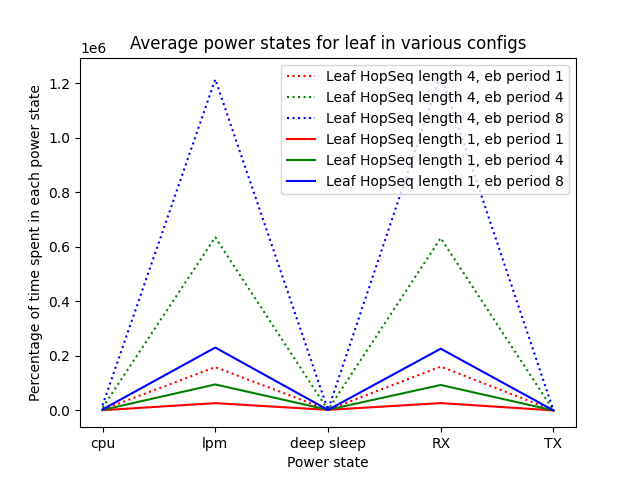
\includegraphics[width=.48\textwidth,keepaspectratio]{figures/leaf_powerstates}
	\caption{The average connection times per configuration. X axis is the configuration (hopping sequence length, EB period), Y axis in seconds}
	\label{fig:t2root}
\end{figure}

\figref{fig:t2root} shows the root power states, for each configuration. Again, we see roughly identical power state distribution for each configuration. It is notably different from the leaf power states graph in that the root node spends most of its time in the sleep state. This is to be expected as it already has all the required information to operate efficiently. 

\begin{figure}[htbp]
	\centering
	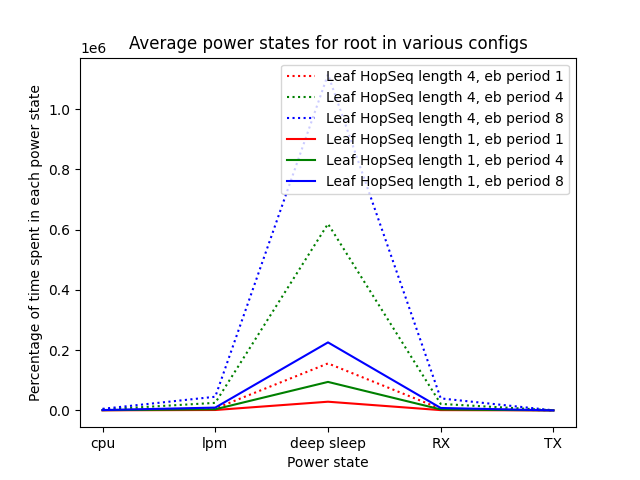
\includegraphics[width=.48\textwidth,keepaspectratio]{figures/root_powerstates}
	\caption{Seconds needed to successfully connect, on average, per configuration}
	\label{fig:t2times}
\end{figure}
\figref{fig:t2times} shows the required connection times for each configuration. It clearly indicates that the length of the hopping sequence is a dominating factor in the estimation of TSCH association times.


\subsection{Conclusion}
We have shown that the hopping sequence does indeed impact the association time more than the EB period does, supporting previous research \cite{JoinProcess}. 


\subsection{Future Work}
\subsubsection{Full measurements} 
As discussed in \secref{sec:t2_discl}, we have severely limited the scope of this analysis because of an oversight on our part. This oversight must be corrected in future work in order to confirm the tentative results we've presented here. 
\subsubsection{Additional parameters}
Considering other variables, for example, TSCH\_CONF\_ASSOCIATION\_POLL\_FREQUENCY would be interesting. There are many variables that have an impact on the TSCH association process and our analyses do not offer thorough coverage. 

\section{Impact of distance on energy consumption and network reliability}
\label{section:task3}
\subsection{Introduction}

In this section, we look at the impact seperation between two nodes has on the energy use of the nodes and the reliability of the TSCH layer. We consider 4 distances and 3 TX power levels and evaluate the performance based on the device power states (recorded using Energest) and the delivery rate (recorded using necessary retransmission count on MAC layer). 

\subsection{Configuration} 
For the most part, the default configuration of Contiki-NG is used. Any non-default values we've used, as well as other important details, are discussed here.

\subsubsection{Network topology}
We study a two-node TSCH network. Both nodes are Zolertia RE-mote (Rev. B) boards. One will act as the TSCH coordinator, the other as a leaf node. In all tests performed in this section, the traffic is sent from the leaf node to the root node. 

The nodes always remain within line of sight, at equal heights (elevated 1 meter above the ground). The only physical parameter being varied (other than those outside our control) is the distance between them. For our range analysis, we consider four distances: 1 meter, 10 meters, 50 meters and 100 meters. The node positions at each distance were marked, to ensure they were positioned as reliably as possible.

\figref{fig:distance} shows a satellite image of where the measurements were taken. In this image, white and red dots were added marking the locations. The white dot is the location the static root node was placed. Then each red dot marks one of the locations that the leaf was placed in to perform our testing. 

\begin{figure}[htbp]
	\centering
	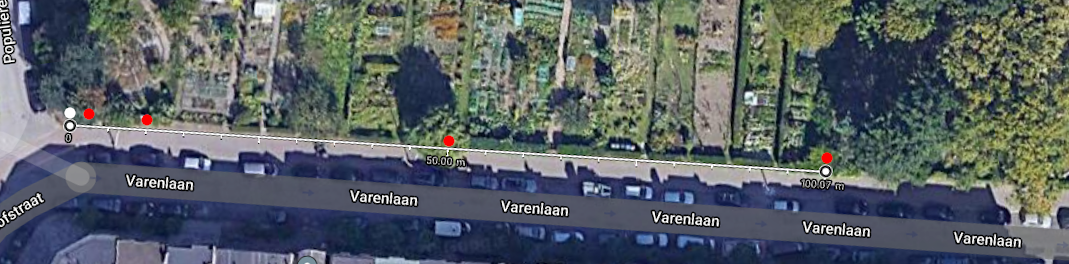
\includegraphics[width=.48\textwidth,keepaspectratio]{figures/distance}
	\caption{Satellite image of the location the measurements were made}
	\label{fig:distance}
\end{figure}

\subsubsection{TX power}
\label{section:txpower}

For each distance in the experiment, we also consider the impact of the TX power parameter. This value sets the intensity of the signal transmission. A larger TX power value leads to increased energy consumption\cite{AccurateEnergyTSCH}. The amount of extra energy consumed by varying this value is left outside the scope of this study, because our study is limited to observing time spent in each energy state. We do have access to the required hardware to accurately determine how much power the device is drawing in any given energy state. The associated current draw for each energy state (used to compute final energy consumption values) is obtained through spec sheets or device profiling results (see \tabref{tab:CurrentConsumption}). We consider 3 distinct values for this parameter: 7 dBm, 0 dBm and -7 dBm. 


\subsubsection{Traffic characteristics}
\label{section:trafficchar}
The traffic is uniform, 1 packet is sent per second. The packets contain 64 bytes of data. The packet size was chosen because 64 bytes is sufficiently large to contain sensor measurement data while remaining small enough to be transmitted over the TSCH layer without fragmentation. Each experiment will send 60 packets so that we may average the performance for each parameter set over that data. 



\subsubsection{TSCH schedule}
\label{section:tschschedule}

We use a very simple schedule for our experiments. There is a single advertising-only cell at (0, 0) and a cell used to transmit our data packets at (1, 1). The (0, 0) cell is used for beacons, so that the leaf node can join the network. It is not used for any of our measurements. All data we collect is sent on the (1, 1) cell. That cell is configured as a transmit-only (to the coordinator) cell in the leaf node and a receive-only (from the leaf) cell in the coordinator node. This setup is illustrated in \figref{fig:TSCHSchedule}. The size of the schedule is left as its default value, that is, 7 slots per frame, 4 channels.

\begin{figure}[htbp]
	\centering
	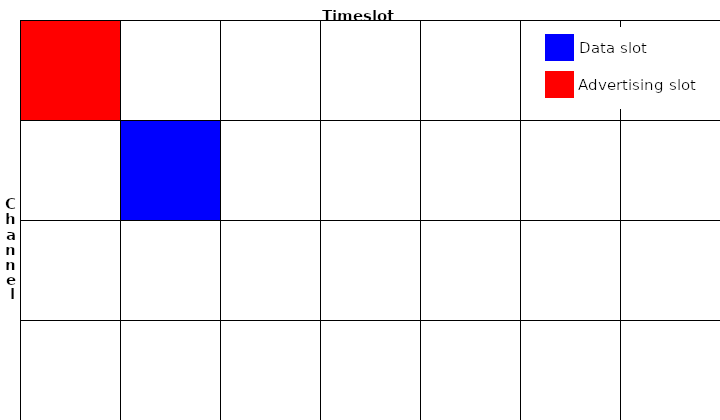
\includegraphics[width=.48\textwidth,keepaspectratio]{figures/tsch_schedule.png}
	\caption{TSCH Schedule as used in the range analysis experiments}
	\label{fig:TSCHSchedule}
\end{figure}

\subsubsection{Network stack}
\label{section:netstack}

For these experiments, most of the default Contiki-NG network stack has been disabled. We're interested in the performance of TSCH, so our experiments interact directly with the MAC layer. To facilitate this, Contiki-NG is built with the following Makefile variables set: 
\begin{itemize}
{
\small
\item MAKE\_MAC=MAKE\_MAC\_TSCH
\item MAKE\_NET=MAKE\_NET\_NULLNET
\item MAKE\_ROUTING=MAKE\_ROUTING\_NULLROUTING
}
\end{itemize}

MAKE\_MAC\_TSCH configures the build system to build the TSCH MAC layer. MAKE\_NET\_NULLNET and MAKE\_ROUTING\_NULLROUTING essentially disable their respective functionalities. Placeholder functions (no side-effects, always return success) are defined in Contiki-NG, but these are not used by our implementation. 

\subsubsection{Preprocessor definitions}

The following values are defined in the preprocessor (some through Makefile, others through header definitions) in order to configure the behavior we want. Each parameter is briefly explained below.

\label{section:preprocessdef}
\begin{itemize}
{
\small
\item ENERGEST\_CONF\_ON=1\\ Enable the energest package to allow analysis of power use. 
\item TSCH\_SCHEDULE\_CONF\_WITH\_6TISCH\_MINIMAL=0\\ Disable creation of a default TSCH schedule. Instead we create our own, as described in \secref{section:tschschedule}.
\item LLSEC802154\_CONF\_ENABLED=0\\ Disable Link Layer security.
\item TSCH\_CONF\_JOIN\_SECURED\_ONLY=0\\ Allow TSCH to join unsecured networks.
}
\end{itemize}



\subsection{Results}


\subsubsection{Network reliability}
The PHY delivery ratio for packets is somewhat interchangeable for all TX powers at low distances. This is clear from \figref{fig:txattempts}. At higher distances, though, it becomes clear that the lower TX power struggles significantly more than the high TX power. In fact, while the TX power set to 7 dBm at 100 meters manages to deliver 100\% of packets, the -7 dBm TX power setting fails to do so. At 50m, it failed to deliver 2 out of 60 packets. At 100 meters, that shot up to 19/60. It is clear, then, that for two nodes that are separated by 100 meters, a TX power setting of -7 dBm is woefully insufficient. 


\begin{figure}[htbp]
	\centering
	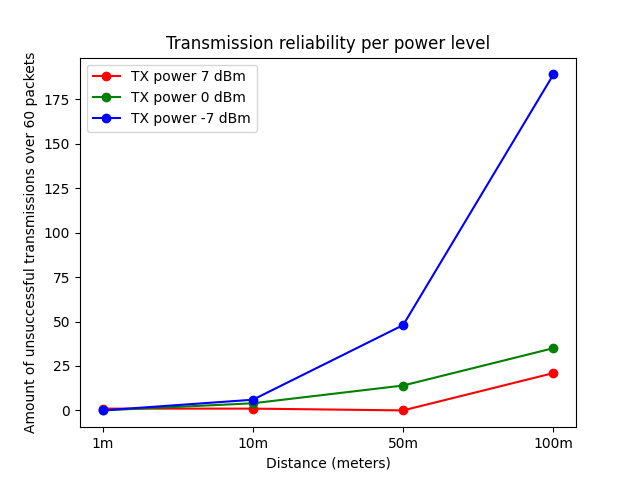
\includegraphics[width=.48\textwidth,keepaspectratio]{figures/retransmissions}
	\caption{Overview of amount of transmission attempts are made on average to send a single packet}
	\label{fig:txattempts}
\end{figure}


This is also clearly visible in the packet latencies, as seen in \figref{fig:averagelatencies}. Clearly, as distance increases, so does the experienced packet latency. It is important to note that \figref{fig:averagelatencies} does not account for packets that did not arrive - it simply leaves them out of the calculation. This was done because no meaningful latency can be ascribed to a packet that did not arrive correctly. It clearly shows that as the distance increases and/or TX power decreases, the latency increases. The degree to which that happens, though, is underrepresented due to this fact.

\begin{figure}[htbp]
	\centering
	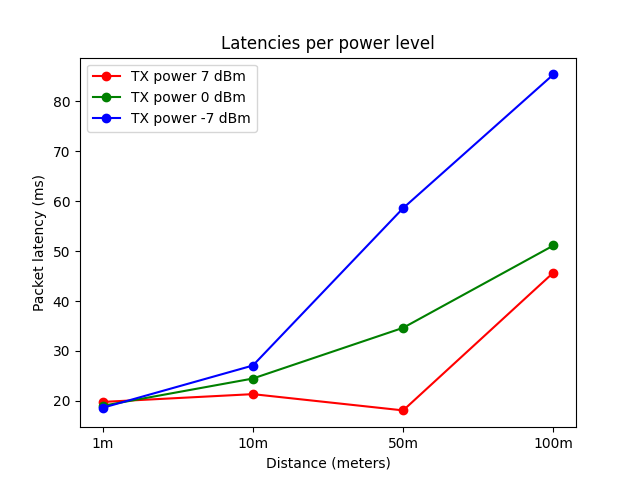
\includegraphics[width=.48\textwidth,keepaspectratio]{figures/latencies}
	\caption{The average packet latencies for each distance/power combination}
	\label{fig:averagelatencies}
\end{figure}

\subsubsection{Energy use}

\figref{fig:leaf_allstates} shows what percentage of time the leaf node spends in each power state in each of the experiments. The energy states are remarkably similar in all cases. The power states at 100m, -7 dBm are slightly offset from the rest of them. Presumably, because of the extra necessary re-transmissions, both the CPU and the radio are not able to sleep, or deep sleep, quite as often as they otherwise would. With the difference being so small, though, it is clear that the code we wrote has minimal impact on the device power states. 

\begin{figure}[htbp]
	\centering
	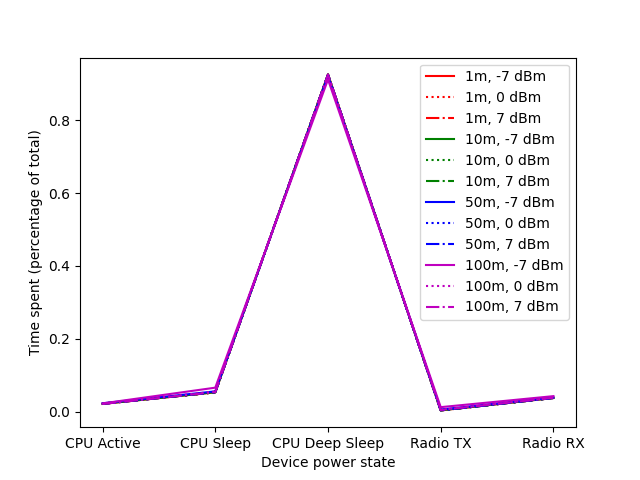
\includegraphics[width=.48\textwidth,keepaspectratio]{figures/leaf_allstates}
	\caption{Power states for the leaf node, over all experiment setups}
	\label{fig:leaf_allstates}
\end{figure}

In \figref{fig:leaf_radiostates} we zoom in on the radio power states (RX and TX). Here it is clear that the large distance, low TX power configuration uses relatively more radio time than the others, both RX and TX. That both increase seems intuitively correct, as retransmissions being necessary would require additional radio awake time. It is interesting that the RX time seems to increase relatively more than the TX time. This could be explained by the fact that when a node receives the ACK for a packet it has sent, it no longer needs to listen, allowing it to shut down the radio sooner. When the transmission fails, the radio has to be on for a longer period of time, causing a larger discrepancy. 

\begin{figure}[htbp]
	\centering
	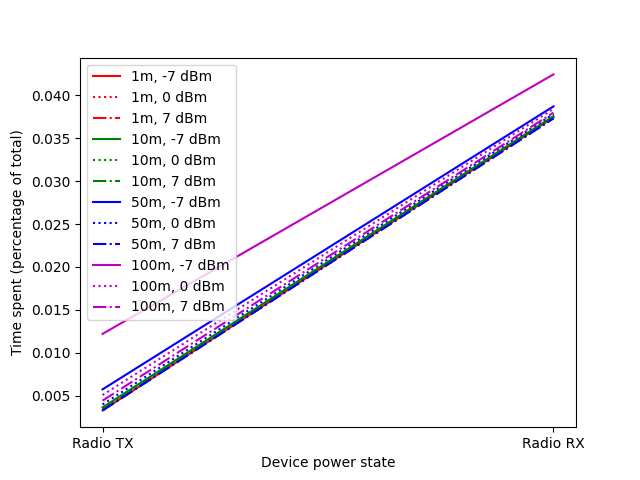
\includegraphics[width=.48\textwidth,keepaspectratio]{figures/leaf_rx_tx}
	\caption{Power states for the leaf node, zoomed in on radio states only}
	\label{fig:leaf_radiostates}
\end{figure}


We also look at the root node's power results, in \figref{fig:root_allstates} and \figref{fig:root_radiostates}. These are even more similar than the leaf node's are, nearly identical in all cases. This is expected, though. The root application we are using does not, itself, transmit data. Rather, it only records its own energy state information when data is received from the leaf node. A very large majority of the time, the root application is simply sleeping. 
\begin{figure}[htbp]
	\centering
	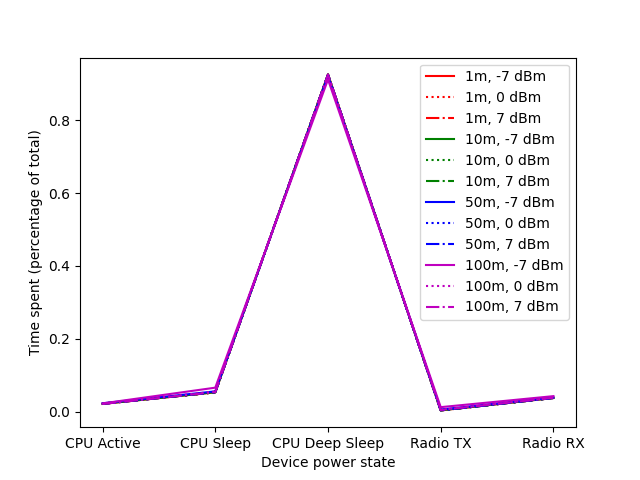
\includegraphics[width=.48\textwidth,keepaspectratio]{figures/root_allstates}
	\caption{Power states for the leaf node, over all experiment setups}
	\label{fig:root_allstates}
\end{figure}
\begin{figure}[htbp]
	\centering
	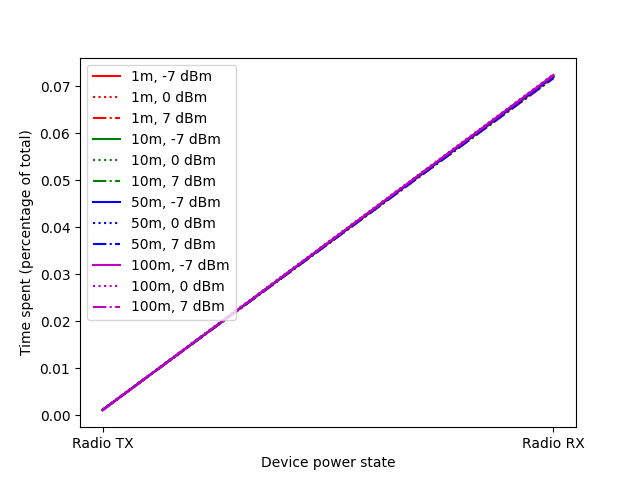
\includegraphics[width=.48\textwidth,keepaspectratio]{figures/root_rx_tx}
	\caption{Power states for the leaf node, zoomed in on radio states only}
	\label{fig:root_radiostates}
\end{figure}


We use the values obtained through device profiling in \tabref{tab:CurrentConsumption} to estimate the node power use. This computation does not take into account the impact of the varied TX power parameter. As discussed in \secref{section:txpower}, it is not feasible for us to correctly assess power use while taking that parameter into account. 

In order to maintain clarity despite this restriction, we keep separate counts for the power used by the radio and the power used by the processor. It is thus important to note that for all figures in \tabref{tab:t3_powerresults}, the radio power use results are not quite as accurate as they could be. Both -7 dBm and 0 dBm values are higher than they should be (-7 dBm more so than 0 dBm), while 7 dBm's stated values are lower than they should be (the source of our data (\cite{EnergyConsumption}) does not mention changing the TX power, so presumably it was left at its default value of 3 dBm). 

It is clear that, for the most part, the power use is close to identical for every considered scenario. As the distance increases, a slight increase in radio power use can be seen in all cases. More so in the low TX power cases. Given the results seen in \figref{fig:leaf_radiostates} and \figref{fig:root_radiostates}, that is to be expected. 

Each experiment transmitted 30720 bits (64 bytes * 60 packets * 8 bits per byte). Using that fact, we can compute the amount of energy per kilobit that was transmitted or received (for leaf and root, respectively). These numbers can be found in \tabref{tab:t3_powerperkilobit}. 


\subsection{Conclusion}

The software we implemented barely influenced the power state the device was in. CPU-wise, this matches our expectations. Our program is written such that there is minimal computation required and most of the time our process sleeps, waiting for events to occur. In the case of the radio, the power use increases when more packets need to be sent. In our use-case, that is the case when retransmissions occur. If no retransmissions occur, the data sent is always the same. 

We've found that the TSCH layer manages good reliability over a distance of 100m, if the TX power parameter is set high enough. For a lower value for the TX power parameter, performance is lacklustre. Clearly there is a balance to be found between adequate performance and impact on the battery life. A TX power parameter that is set unnecessarily high will impact the battery life of a node simply by requiring more power per transmission, whereas a lower value will require more power because retransmissions are more likely. For any given distance, and environment noise level, the 

\section{Future Work}
\label{section:futurework}

\subsubsection{Varied packet size}
In this study, we've only looked at the performance characteristics of the network at various distances for packets carrying 64 bytes of data payload. An interesting follow-up might be the analysis of how the results change when the packet size is varied as well. A sensor network doing less complex measurements could definitely get by with smaller packets, for example. Smaller packets lead to shorter transmission times. This may reduce the error rate during transmission and thus could potentially achieve the same reliability at a lower TX power. 

\subsubsection{Individually varied TX power}
We've only considered the case where TX power is varied on both nodes. A potentially interesting follow-up to this is to consider the impact varying the parameter on one of the nodes has. This would clarify if, in order to ensure satisfactory network performance, TX power must be increased for all nodes or only for some. Our results have shown that larger TX power results in fewer retransmission (at the cost of increased power use per transmission\cite{AccurateEnergyTSCH}), but we've not studied the trade-off in more detail. It is conceivable to have the root node be connected to a power source, while other nodes are running on battery, for example. So an interesting study would be to only increase TX power on the root node and see if (and to what degree) that improves performance the reliability, since its energy consumption is less relevant. 

\printbibliography

\onecolumn

\begin{table}[htbp]
\noindent\makebox[\textwidth]{
\begin{tabular}{c|c|c|c|c|c|c|c}
\multicolumn{2}{c}{\multirow{2}{*}{}} & \multicolumn{2}{c}{-7 dBm} & \multicolumn{2}{c}{0 dBm} & \multicolumn{2}{c}{7 dBm} \\ \cline{3-8}
\multicolumn{2}{c}{}                  & cpu          & radio       & cpu         & radio       & cpu         & radio       \\ \hline
1 meter                       & root  & 0.2050 J     & 0.1367 J    & 0.2051 J    & 0.1364 J    & 0.2048 J    & 0.1363 J    \\ \cline{2-8}
                              & leaf  & 0.1936 J     & 0.0760 J    & 0.1946 J    & 0.0759 J    & 0.1939 J    & 0.0759 J    \\ \hline
\multirow{2}{*}{10 meters}    & root  & 0.2053 J     & 0.1371 J    & 0.2060 J    & 0.1378 J    & 0.2048 J    & 0.1365 J    \\ \cline{2-8}
                              & leaf  & 0.1942 J     & 0.0770 J    & 0.1949 J    & 0.0765 J    & 0.1942 J    & 0.0759 J    \\ \hline
\multirow{2}{*}{50 meters}    & root  & 0.2054 J     & 0.1372 J    & 0.2063 J    & 0.1376 J    & 0.2053 J    & 0.1365 J    \\ \cline{2-8}
                              & leaf  & 0.1963 J     & 0.0829 J    & 0.1939 J    & 0.0780 J    & 0.1940 J    & 0.0758 J    \\ \hline
\multirow{2}{*}{100 meters}   & root  & 0.2065 J     & 0.1382 J    & 0.2060 J    & 0.1382 J    & 0.2052 J    & 0.1373 J    \\ \cline{2-8}
                              & leaf  & 0.2001 J     & 0.1015 J    & 0.1949 J    & 0.0811 J    & 0.1940 J    & 0.0791 J   
                             
\end{tabular} 
}
\label{tab:t3_powerresults}
\caption{Power use for leaf and root nodes in all experiment setups}
\end{table}

\begin{table}[htbp]
\noindent\makebox[\textwidth]{
\begin{tabular}{c|c|c|c|c|c|c|c}
\multicolumn{2}{c}{\multirow{2}{*}{}} & \multicolumn{2}{c}{-7 dBm} & \multicolumn{2}{c}{0 dBm} & \multicolumn{2}{c}{7 dBm} \\[3pt] \cline{3-8}
\multicolumn{2}{c}{}                  & cpu          & radio       & cpu         & radio       & cpu         & radio       \\[3pt] \hline
1 meter                       & root  & 6.833 $\frac{mJ}{kbit}$ & 4.557 $\frac{mJ}{kbit}$ & 6.837 $\frac{mJ}{kbit}$ & 4.547 $\frac{mJ}{kbit}$ & 6.827 $\frac{mJ}{kbit}$ & 4.543 $\frac{mJ}{kbit}$ \\[3pt] \cline{2-8}
                              & leaf  & 6.453 $\frac{mJ}{kbit}$ & 2.53 $\frac{mJ}{kbit}$ & 6.487$\frac{mJ}{kbit}$ & 2.53 $\frac{mJ}{kbit}$ & 6.463 $\frac{mJ}{kbit}$ & 2.53 $\frac{mJ}{kbit}$ \\[3pt] \hline
\multirow{2}{*}{10 meters}    & root  & 6.843 $\frac{mJ}{kbit}$ & 4.570 $\frac{mJ}{kbit}$ & 6.867 $\frac{mJ}{kbit}$ & 4.593 $\frac{mJ}{kbit}$ & 6.827 $\frac{mJ}{kbit}$ & 4.55 $\frac{mJ}{kbit}$ \\[3pt] \cline{2-8}
                              & leaf  & 6.473 $\frac{mJ}{kbit}$ & 2.567 $\frac{mJ}{kbit}$ & 6.497 $\frac{mJ}{kbit}$ & 2.55 $\frac{mJ}{kbit}$ & 6.473 $\frac{mJ}{kbit}$ & 2.53 $\frac{mJ}{kbit}$ \\[3pt] \hline
\multirow{2}{*}{50 meters}    & root  & 6.847 $\frac{mJ}{kbit}$ & 4.573 $\frac{mJ}{kbit}$ & 6.877 $\frac{mJ}{kbit}$ & 4.587 $\frac{mJ}{kbit}$ & 6.843 $\frac{mJ}{kbit}$ & 4.55 $\frac{mJ}{kbit}$ \\[3pt] \cline{2-8}
                              & leaf  & 6.543 $\frac{mJ}{kbit}$ & 2.763 $\frac{mJ}{kbit}$ & 6.463 $\frac{mJ}{kbit}$ & 2.6 $\frac{mJ}{kbit}$ & 6.467 $\frac{mJ}{kbit}$ & 2.527 $\frac{mJ}{kbit}$ \\[3pt] \hline
\multirow{2}{*}{100 meters}   & root  & 6.883 $\frac{mJ}{kbit}$ & 4.607 $\frac{mJ}{kbit}$ & 6.867 $\frac{mJ}{kbit}$ & 4.607 $\frac{mJ}{kbit}$ & 6.84 $\frac{mJ}{kbit}$ & 4.577 $\frac{mJ}{kbit}$ \\[3pt] \cline{2-8}
                              & leaf  & 6.67 $\frac{mJ}{kbit}$ & 3.383 $\frac{mJ}{kbit}$ & 6.497 $\frac{mJ}{kbit}$ & 2.703 $\frac{mJ}{kbit}$ & 6.467 $\frac{mJ}{kbit}$ & 2.637 $\frac{mJ}{kbit}$
\end{tabular}
}
\label{tab:t3_powerperkilobit}
\caption{Power use for leaf and root nodes in all experiment setups}
\end{table}
\twocolumn


\end{document}
